\usetikzlibrary{arrows.meta,calc,patterns,shapes}
\providecommand{\computer}{%
    
\includegraphics[width=1cm,alt={computer}]{../common/Noun_project_216.pdf}
}
\providecommand{\switch}{%
    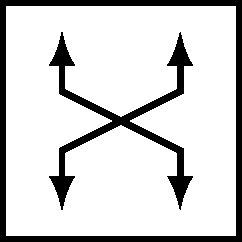
\includegraphics[width=0.9cm,alt={switch}]{../common/fig-switch.pdf}
}
\providecommand{\bigswitch}{%
    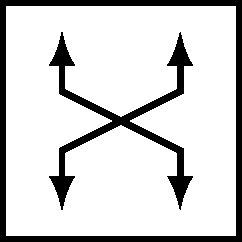
\includegraphics[width=1.4cm,alt={switch}]{../common/fig-switch.pdf}
}
\providecommand{\router}{%
    
\includegraphics[width=0.9cm,alt={router}]{../common/fig-router.pdf}
}



\begin{frame}\frametitle{flows / packets}
\myalttext{
\begin{tikzpicture}
\tikzset{
    connect one/.style={draw,very thick,-Latex},
    computer/.style={inner sep=0mm,outer sep=0mm,execute at begin node={\computer}},
    switch/.style={inner sep=0mm,outer sep=0mm,execute at begin node={\switch}},
    big switch/.style={inner sep=0mm,outer sep=0mm,execute at begin node={\bigswitch}},
    packet/.style={minimum width=.4cm,minimum height=0.2cm,inner sep=0mm,outer sep=0mm,draw},
    packet lg/.style={minimum width=.6cm,minimum height=0.2cm,inner sep=0mm,outer sep=0mm,draw},
    c1c2/.style={fill=violet!40,draw=black,thin,slidealt=<2>{thick,draw=red}},
}
\node[computer] (c1) at (-5, 1) {};
\node at (c1) {1};
\node[big switch] (s1) at (-2,-.5) {};
\node[big switch] (s2) at (2,.5) {};
\node[computer] (c2) at (6, 2) {};
\node at (c2) {2};
\draw[connect one] (c1) -- (s1)
    node[above=0.05cm,sloped,packet,c1c2,pos=0.1] {}
    node[above=0.05cm,sloped,packet lg,c1c2,pos=0.5] {}
    node[above=0.05cm,sloped,packet,c1c2,pos=0.8] {};
\draw[connect one] (s1) -- (s2)
    node[above=0.05cm,sloped,packet,c1c2,pos=0.3] {}
    node[above=0.05cm,sloped,packet,c1c2,pos=0.8] {};
\draw[connect one] (s2) -- (c2)
    node[above=0.05cm,sloped,packet,c1c2,pos=0.2] {}
    node[above=0.05cm,sloped,packet lg,c1c2,pos=0.6] {};
\node[packet,c1c2,anchor=north east] at ([yshift=-.1cm,xshift=-.1cm]s1.north east) {};
\node[packet lg,c1c2,anchor=north east] at ([yshift=-.3cm,xshift=-.1cm]s1.north east) {};
%
\node[packet,c1c2,anchor=north east] at ([yshift=-.1cm,xshift=-.1cm]s2.north east) {};
\node[packet,c1c2,anchor=north east] at ([yshift=-.3cm,xshift=-.1cm]s2.north east) {};
\node[packet,c1c2,anchor=north east] at ([yshift=-.5cm,xshift=-.1cm]s2.north east) {};
\coordinate (box loc) at (-4, -1.5);
\tikzset{
    explain box/.style={
        overlay,draw=red, align=left, very thick, anchor=north west,at=(box loc)
    },
}
\begin{visibleenv}<1>
\node[explain box] {
    \textit{\myemph{flow}} of data between two machines \\
    ~ \\
    \textit{flow} is very general term \\
    will depend on context how it relates to \\
    connections, sockets, etc.
};
\end{visibleenv}
\begin{visibleenv}<2>
\node[explain box] {
    \textit{\myemph{flow}} of data between two machines \\
    ~ \\
    possibly divided up into pieces, \\
    called \textit{\myemph{packets}}, \textit{\myemph{frames}}, \textit{\myemph{segments}} \\
    (which name is best depends on context)
};
\end{visibleenv}
\end{tikzpicture}
}{
Diagram showing data going via two switches from machine 1 to machine 2. This is labeled as a *flow*. Flows can be divided up into pieces
called packets, frames, or segments (which name is best depends on context). The diagram shows the flow being divided into
variably-sized packets, some of which are in transit on links between nodes and some of which are in queues on the switches.
}
\end{frame}

\begin{frame}{flows}
\begin{itemize}
\item flow = data flowing `together' across a network
\item often different ways of dividing data into flows
    \begin{itemize}
    \item if we need precision, we'll define it more precisely
    \end{itemize}
\item flow divided into packets/frames/segments
    \begin{itemize}
    \item best name depends on which layer we're looking at
    \item won't be picky about it because the world isn't
    \end{itemize}
\end{itemize}
\end{frame}
